
\chapter{Plenoptic De-blurring}
\label{chap:plenoptic_deblurring}

\section{Light Field Theory}

%Side Note
%The first practical work using light fields dates back to a photographic technique known as ‘Integral Photography’, developed by Gabriel Lipmann in 1908.
%Lipmann’s technique involved placing an array of lenses over a piece of film.
%The film was then exposed to a scene, encoding 3D information through the lens pattern. 
%By reversing this process (projecting light through the film, then through an identical lens array), the first 3D pictures were created.
%Modern techniques allow Lipmann’s lens arrays to be printed on a surface, creating what is commonly known as ‘holographic pictures’ that morph and change as the viewer’s perspective changes.
%GIVE MORE INFORMATION ON INTEGRAL PHOTOGRAPHY.
%The ability to create a 3D display in this manner (without extra viewing devices such as 3D glasses) is known as auto-stereoscopic imaging.


The light field is a mathematical description of the way light propagates.
Another name for this is the \enquote*{Plenoptic Function}, from the Latin \enquote*{plenus}, meaning full, and \enquote*{optic}, meaning light.
The plenoptic function describes every possible configuration a light ray could ever be in, encompassing the three spatial dimensions, two angular dimensions, temporal changes as well as frequency (colour), phase and polarisation changes.
In most computer vision literature the phase and polarisation elements are ignored, leading to a 7-dimensional definition of the plenoptic function;

\begin{equation}
\label{eq:plenoptic_function}
P = P(V_x, V_y, V_z, \theta, \phi, t, \lambda)
\end{equation}

where $V_x$, $V_y$ and $V_z$ are the spatial dimensions, $\theta$ and $\phi$ are the angular dimensions, $t$ is the temporal dimension and $\lambda$ describes the colour of the ray. 

The plenoptic function in this form was first described by Adelson and Bergen in 1991 \cite{adelson1991plenoptic}.
Adelson and Bergen developed a light field theory by asking the fundamental question \enquote{What can be seen?} They stressed that the plenoptic function is the sole visual communication link between physical objects and the eye.
They also suggested that the function of \enquote*{early vision} in biological and artificial organisms is to sample the derivative of this function along various dimensions such as \enquote*{change in colour with x} or \enquote*{change in brightness with time}.
\hl{GIVE DETAIL ABOUT SAMPLING PLENOPTIC FUNCTION EXAMPLES FROM ADELSON PAPER.}

In modern computer vision literature a number of parameterisations are used to describe the plenoptic function.
These different representations each provide new insights into the information contained in the light field.

\hl{LIGHT SLAB DESCRIPTION AND DISCUSSION.}

\hl{LIGHT TUBE DESCRIPTION AND DISCUSSION.}

\hl{POLAR AND/OR DUAL PLANE DESCRIPTION AND DISCUSSION?}


Traditional cameras generally sample the Light Field along two spatial dimensions (x and y pixel locations) and in the colour dimension (normally with Red, Green and Blue photon collectors), however there are many instances in which sampling more dimensions of the light field would be beneficial. To this end, in 1996 two light field papers were included in the Siggraph conference proceedings; ‘Light Field Rendering’ by Levoy et al. and ‘The Lumigraph’ by Gortler et al \hl{[REFERENCES]}. Both these papers described independent research into means for capturing more information from the plenoptic function. Importantly, both groups made the observation that, while the full plenoptic function is seven dimensional, for a region of space free of occluding objects, one space dimension can be disregarded, and the 3D structure of the scene still fully recovered. \hl{GO INTO MORE DETAIL ABOUT OCCLUSION FREE SPACE SIMPLIFICATION HERE}. This approximation is the basis for most modern light field cameras sampling in four dimensions, and paved the way for the creation of the first practical light field cameras.

All physical cameras (or eyes) can only ever observe a small subset (various ‘slices’) of the ambient light field. As an example, consider the human visual system. The human visual system takes several million samples from the angular dimensions, three points from the lambda dimension (roughly corresponding to the frequencies known as ‘Blue’, ‘Green’ and ‘Red’) and only two samples from the Vx dimension (one each for the left and right eyes). In addition to this, the distribution of sample points is not always linear. The cone cells responsible for detecting colour in the human eye are much more populous in the fovetal region near the centre of the eye, while rod cells that operate in low-light conditions are clustered around the outer edges of the retina.

The work done by Gortler and Levoy (et al.) demonstrated it was possible to capture 4D light field information using a traditional camera sensor with some modifications. While there is active research in developing angle-sensitive pixels, modern light field cameras typically encode angular ray information by mapping ray angles to locations on a traditional 2D camera sensor. Thus, regular spatial resolution is directly traded to gain angular resolution.

For example the Lytro light field camera used in this paper has an 11 mega-pixel sensor chip, however a spatial and angular resolution of only 1080x1080 and 10x10 respectively. The trade-off between angular resolution and spatial resolution is unavoidable when using this technique, and the choice of angular and spatial resolutions limit the functions that can be performed with the captured light field.
\hl{GIVE EXMPLES OF HOW NOT ALL LIGHT FIELDS ARE EQUAL.
DISCUSS THE BENEFITS/DRAWBACKS OF THE LYTRO CAMERA CONFIGURATION}.
4D light field sampling has also been performed using multiple traditional cameras separated spatially in a grid, or separated temporally.

\hl{GO INTO MORE DETAIL ABOUT LYTRO CAMRERA AND BRIEFLY COMPARE LYTRO WITH RAYTRIX AND OTHER LF CAMERAS (STANFORD MULTI CAMERA ARRAY).
ALSO DISCUSS SYNTHETIC LIGHT FIELD CREATION AND GIVE EXMAPLES.
HIGHLIGHT BENEFITS AND DRAWBACKS OF SYNTHETIC LIGHT FIELDS VS REAL TEST DATA.
MENTION THE APPEARANCE OF LIGHT FIELD CAMERAS ON MOBILE PHONES.
MENTION ANDROID LF CAMERA.
}

Mapping of ray angles to the 2D camera plane is typically done by placing either a lenslet or mirror array, or a cosine pinhole mask within the light ray path. These approaches are functionally equivalent, however each has disadvantages and benefits. A lenslet or mirror array is di cult to machine and requires custom hardware and precision positioning. On the other hand, a pinhole array can be added to some modern cameras with little modification, however blocks a large majority of the incoming light, thus requiring longer exposure times and increasing the likelihood of motion blurring.

\hl{
2 OR 3 PARAGRAPHS ABOUT LOW RESOLUTION AND LIGHT FIELD SUPER RESOLUTION PAPER.

POSSIBLY 2-3 MORE PARAGRAPHS ABOUT RECENT LIGHT FIELD RESEARCH AND DEVELOPMENTS.

2 SUMMARISING PARAGRAPHS BRINGING ALL OF THIS INFORMATION BACK TO MY THESIS – HIGHLIGHTING WHAT PARTS I’M GOING TO BE USING, WHAT LF SYMBOLS AND CONVENTIONS I’LL BE USING ETC.
}


\section{Motion Blur Formation}
\label{sec:motion_blur_formation}

Motion blur occurs in any non-theoretical camera due to a finite exposure time, combined with the presence of camera, or object motion within the scene.
This is distinct from focal blur, which is a by-product of the optical behavior of any camera aperture larger than an infinitesimal point (a perfect pinhole aperture).
If the camera or objects within the scene move during the exposure time, light rays from the scene that would otherwise be focused on a single photosite are distributed across multiple photosites.
The objects within the scene therefore become \enquote*{smeared} across several pixels in the resultant image \hl{(figure XXXX)}.

\hl{[Figure XXXX here showing camera integration over time, and blur occurring]}

In a projective geometry imaging system --such as most cameras-- blur from camera or object linear motion in any plane perpendicular to the optical axis appears as a linear \enquote*{smear} in the image x or y directions.
This \enquote*{smear} is known as a Point Spread Function (PSF), as it describes the spreading that occurs to a perfect point source within the scene.
This is analogous to the impulse response of a frequency domain system; in this case the system is the optical apparatus, and the impulse is the point source in the scene.

Movement along the optical axis (as compared to movement perpendicular to the optical axis) results in a radial point spread function, while camera or object rotation creates a radial point spread function centered at the origin of the rotation \hl{(figure XXXX)}.
In all cases, the degree of blur varies with the distance from the camera to the object moving.
In this thesis, for the sake of simplicity, we focus on de-blurring linear motion blur induced through camera motion.

\hl{[Figure XXXX here, showing camera or object motion perpendicular to and along the optical axis]}

In order to de-blur light field data, it was necessary to quantitatively describe the way motion blur forms in a camera.
Specifically, it was necessary to derive an equation describing the way a motion blur Point Spread Function varied with respect to scene depth.
To do this, the homogeneous projective geometry equation was used;

\begin{equation}
\label{eq:camera_projection_unexpanded}
k \boldsymbol{x} = \boldsymbol{K} \left[~\boldsymbol{R}~|~\boldsymbol{t}~\right] \boldsymbol{X}
\end{equation}

where $k$ is the homogeneous scaling constant, $\boldsymbol{x}$ is the image-space point location, $\boldsymbol{K}$ is the so-called \enquote*{camera intrinsic matrix} that accounts for camera distortions, $\boldsymbol{R}$ is the 3x3 camera rotation matrix,  $\boldsymbol{t}$ is the camera's 3x1 world-frame translation vector and $\boldsymbol{X}$ is the world-frame point location.
\hl{Figure XXXX} shows the geometry involved in equation \ref{eq:camera_projection_unexpanded}.

\hl{[Figure XXXX]}

Expanding the matrix and vector terms, equation \ref{eq:camera_projection} is reached.

\begin{equation}
\label{eq:camera_projection}
k
\begin{bmatrix}
x \\
y \\
1 \\
\end{bmatrix}
=
\begin{bmatrix}
\alpha && s && u_0 \\
0 && \beta && v_0 \\
0 && 0 && 1 \\
\end{bmatrix}
\begin{bmatrix}
r_{11} && r_{12} && r_{13} && t_x \\
r_{21} && r_{22} && r_{23} && t_y \\
r_{31} && r_{32} && r_{33} && t_z \\
\end{bmatrix}
\begin{bmatrix}
X \\
Y \\
Z \\
1
\end{bmatrix}
\end{equation}

Here the intrinsic matrix $\alpha$ and $\beta$ terms are the camera focal length, scaled to be in units of x and y pixels respectively, $s$ is a shearing factor that describes the shear of the camera sensor (see Figure \ref{fig:intrinsic_shear}) and $u_0$ and $v_0$ are the x and y pixel locations of the optical axis of the camera.

\begin{figure}[h]

\centering


\includegraphics[width=4cm]{pixel_shear.pdf}

\caption[Camera intrinsic matrix shear term]{Camera intrinsic matrix shear term description, $s = \beta\tan(\theta)$. Figure from \cite{pollefeys2002visual}}
\label{fig:intrinsic_shear}

\end{figure}

Assuming the world frame coincides with the camera location and orientation, and assuming linear, horizontal camera motion at velocity $v_c$ meters per second with an exposure time of $t_e$ seconds, the blur width of a point source in the scene can be derived;

\begin{align}
w &= \left| x_1 - x_2 \right| \notag \\
&= \left| \left( \frac{\alpha + s + u_0}{Z} \right) X_1 - \left( \frac{\alpha + s + u_0}{Z} \right) X_2 \right| \notag \\
&= \left| \left( \frac{\alpha + s + u_0}{Z} \right) \left(\frac{- v_c t_e}{2}\right) - \left( \frac{\alpha + s + u_0}{Z} \right) \left(\frac{v_c t_e}{2}\right) \right| \notag \\
\label{eq:blur_width_full}
&= \left( \frac{\alpha + s + u_0}{Z} \right) v_c t_e
\end{align}

Finally, if we then assume square sensor pixels with no sensor skew, and an aligned optical axis, equation \ref{eq:blur_width_full} simplifies to

\begin{equation}
\label{eq:blur_width_simple}
w = \frac{f}{Z} v_c t_e
\end{equation}

Where $f$ is the focal length of the camera.
This equation describes the width of the linear motion blur created by a point source at depth $Z$ within the scene for a moving camera.
Note that the blur width is proportional with the camera focal length, velocity and exposure time, and inversely proportional with depth.
The inverse relation with scene depth correlates with the intuitive expectation; objects further away translate less in an image when the camera moves.
Equation \ref{eq:blur_width_simple} can be thought of as describing a 3D point spread function with $x$, $y$ and $Z$ as the dimensions.
This is shown visually in Figure \ref{fig:psf_3d}.


\begin{figure}[h]

\centering

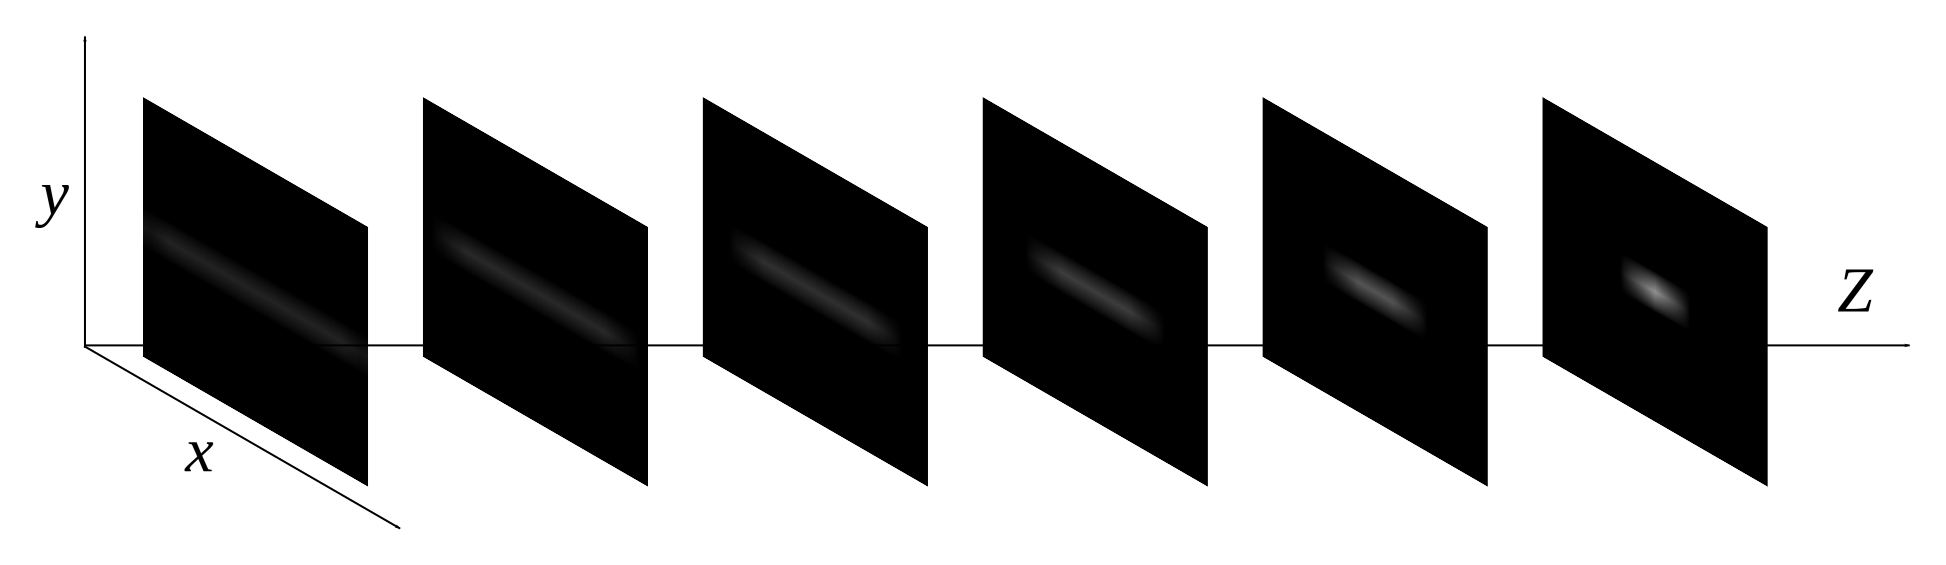
\includegraphics[width=\textwidth]{psf_3d.pdf}

\caption[Visualisation of a 3D Point Spread Function]{Visualisation of a 3D Linear Motion Point Spread Function, with $x$, $y$ and $Z$ as the dimensions}
\label{fig:psf_3d}

\end{figure}

Equation \ref{eq:blur_width_simple} was verified experimentally by taking several photos with a Lytro camera at a controlled velocity and measuring the blur width and depth of objects within the scene.
Only the central sub-aperture image from the light field was used for simplicity.
Figure \ref{fig:blur_vs_width} shows the measured results along with the predicted curve.

\begin{figure}[h]

\centering

\caption[Edge blur width vs. Depth]{Edge blur width vs. Depth - Measured, Predicted and $L^{2}$ regression}
\label{fig:blur_vs_width}

\includegraphics[width=\textwidth]{blur_vs_depth.pdf}


\end{figure}

As can be seen, the equation matched the theoretical curve very closely, indicating that equation \ref{eq:blur_width_simple} is a good fit for an individual sub-aperture image within a light field.
This indicates that if the focal length, linear camera velocity and exposure time are known, and if a calibrated depth map can be recovered from the light field, it should be possible to de-blur all sub-aperture images from the light field image at all scene depths.
This is the basis for the light field de-blurring technique developed in this thesis.
As a final note, observe that the above analysis could also be applied to compute the 3D point spread function for a general camera trajectory, provided the trajectory (camera $\boldsymbol{R}$ and $\boldsymbol{t}$ at all times during the exposure) was known.
This possibility is discussed in Chapter \ref{chap:results_and_discussion} (\nameref{chap:results_and_discussion}).


\section{Image De-blurring}

\hl{
Image formation

Sources of degradation during image formation:
 - Optical blur (light diffraction through lens system), Rayleigh criterion
 - Noise (quantum statistical behaviour of light (shot noise) and read noise (electronics / detection device)).
 - Motion induced blur

Image formation in the fourier domain
 - g(x) = f(x) * h(x) -> G(w) = F(w) x H(w)
 - Additive noise

Point Spread Function – Optical system response to a punctual light source
Optical Transfer Function – Fourier transform of the PSF. Describes optical system behaviour in the fourier domain

Simple deconvolution approaches
 - Inverse \& Regularized Inverse filter
 -- Noise amplification
 - Wiener Filter
 --Signal to Noise Ratio

Iterative Deconvolution
 - Least squares estimation (+regularized)
 - Maximum likelihood estimation (Richardson-Lucy)

Unsharp Masking

Blind deconvolution
}

\section{Light Field Depth Estimation}

As shown in section \ref{sec:motion_blur_formation}, de-blurring at all scene depths requires a depth map calibrated to be in real-world units such as meters.
It was found that the Lytro firmware and/or desktop software computes a low-quality depth map from the Lytro Light Field images, returning integer depth values in an unknown or arbitrary unit.
This depth map can be located within the Lytro image storage database and is contained in Lytro image files with the name \enquote*{dm.lfp}.
The \enquote*{lfpsplitter} tool \cite{patel2013lfptools} was used to extract this data into a single-column text file format, after which Matlab was used to reshape this data into a depth map.
To correctly re-shape the data, it had to be read in standard raster order (left to right, top to bottom), with an expected size of 330x330.

Sample points from within the Lytro depth maps were compared with ground truth depth estimates for a range of real-world scenes, with the scene depth ranging up to 8 meters.
Our initial analysis showed that after the rejection of outliers, the Lytro depth response \enquote*{$D$} was a linear function with real-world object depth \enquote*{$Z$}, however the specific linear function varied as the overall scene depth range changed.
For example, scenes with an overall depth range less than 0.5m were found to be a good fit ($R^2 = 0.69$) with the linear function $Z(D) = 0.0291 \times D + 0.2114$, while scenes with a depth range of 0.5-2m were a a good fit ($R^2 = 0.53$) with the function $Z(D) = 0.1436 \times D + 0.8597$.
Figure XXXX shows these results in graph format.

\begin{figure}[h]
\centering
\caption[Real World Depth vs. Lytro Depth Response]{Real-world depth vs. Lytro Depth response. The data has been binned into three categories based on overall scene depth range.}
\label{fig:depth_real_world_vs_lytro_response}
\includegraphics[width=\textwidth]{depth_real_world_vs_lytro_response.pdf}
\end{figure}

It was found experimentally that the Lytro-generated depth maps have a minimum recoverable depth range of \nicetilde5cm and that the presence of glare prevents accurate depth estimation (see Figure \ref{fig:ruler_glare_min_dist}).
Furthermore, it was found that the presence of motion blur or lack of scene structure reduced the quality of the depth map (see Figures XXXX and \ref{fig:blur_corrupts_depth}).
The reduction in quality due to glare is expected due to the lambertian scene assumption made in many light field computational photography algorithms \cite{bishop2009light, liang2011light, baker2003shape} and the reduction is quality due to motion blur or lack of structure suggests the Lytro software is using a dense correlation based depth estimation method.


\begin{figure}
\centering
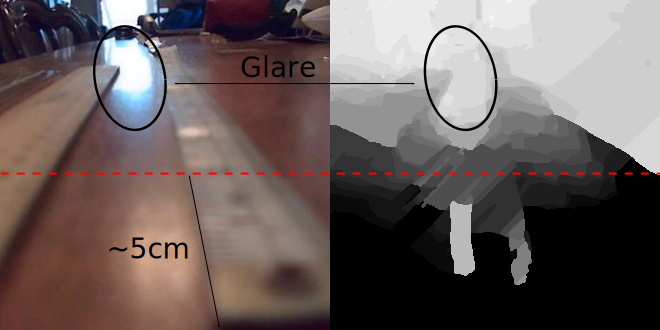
\includegraphics[width=\textwidth]{ruler_glare_min_dist.pdf}
\caption[Minimum depth map distance and the effect of glare]{An example light field image, and the Lytro depth map response. Note the lack of depth data where glare is present, and below Z = 5cm.}
\label{fig:ruler_glare_min_dist}
\end{figure}

\begin{figure}
\centering

\includegraphics[width=\textwidth]{depth_lack_of_structure.png}
\caption[Lack of Scene Structure Corrupts Lytro Depth Estimation]{An example light field image and the Lytro depth response. Note the lack of clear structure in some parts of the image results in large regions without depth variation.}
\label{fig:depth_lack_of_structure}
\end{figure}

\begin{figure}
\centering
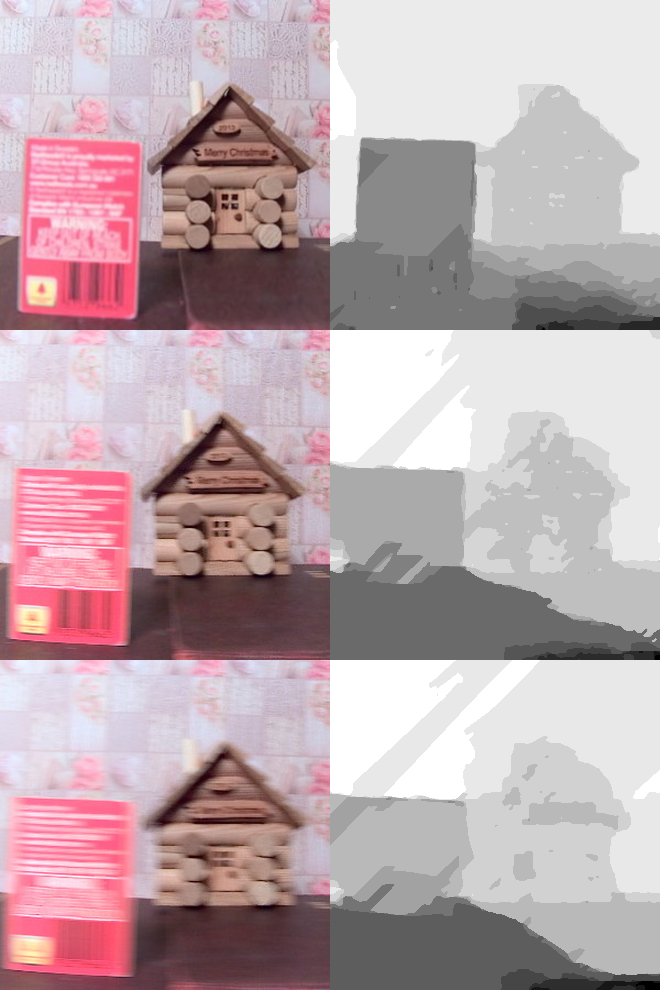
\includegraphics[width=\textwidth]{blur_corrupts_depth.png}
\caption[Motion Blur Corrupts Lytro Depth Estimation]{The same scene photographed three times with the Lytro camera, with progressively more motion blur. Note the reduction in the quality and consistency of the depth response.}
\label{fig:blur_corrupts_depth}
\end{figure}

These findings suggested that if rough knowledge of the scene depth can be obtained, it is possible to calibrate the Lytro depth maps into units of meters, allowing real-world depths to be estimated.
It is suggested that in a real-world application, an infra-red/ultrasound based focal length sensor (as found on many commercial cameras) could be used for this purpose.
Alternately, user-supplied a-priori knowledge of a robotic operating environment, or a user-selected 'scene' setting on a commercial camera (e.g. outdoors, indoors, portrait etc.) could be used here.

The possibility of using other depth estimation methods was explored.
In particular, the Depth from Combining Defocus and Correspondence method by Tao et al. \cite{tao2013depth} was tried.
Using the supplied Matlab source code \cite{tao2013depthwebsite}, depth maps were found to be extremely noisy and completely unusable (see figure \ref{fig:defocus_correspondence_depth}).
It is possible this was due to their code being tuned specifically for their Lytro camera, however due to discovering the more readily available Lytro depth data, this possibility was not explored further.


\begin{figure}[h]
\centering
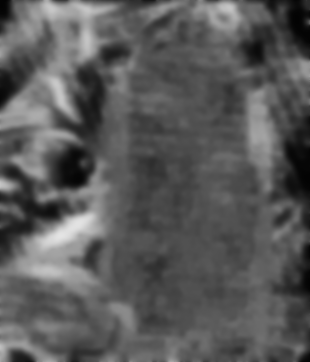
\includegraphics[width=7cm]{defocus_correspondence_depth.png}
\caption[Depth Map from combining Defocus and Correspondence]{An example depth map result from using Defocus and Correspondence by Tao et al. \cite{tao2013depthwebsite} - the input light field is the same as in Figure \ref{fig:depth_lack_of_structure}.}
\label{fig:defocus_correspondence_depth}
\end{figure}
